\documentclass[12pt, a4paper]{book}
\usepackage[a4paper, total={6in, 8in}]{geometry}
\usepackage[english]{babel}
\usepackage{ragged2e}
\usepackage{ragged2e}
\usepackage{fancyhdr}
\usepackage{pageslts}
\usepackage{listings}
\usepackage{color}
\usepackage{graphicx}
\usepackage[hidelinks]{hyperref}
\graphicspath{{images/}}

\def\thesection{\Roman{section}}
\def\thesubsection{\Roman{section}.\Roman{subsection}}
\def\thesubsubsection{\Roman{section}.\Roman{subsection}.\Roman{subsubsection}}

\pagenumbering{arabic}

\pagestyle{fancy}
\fancyhf{}

\lfoot{\small Rev. 1.0}
\rfoot{\small Page \thepage\ of \pageref{LastPage}}

\title{\textbf{{\LARGE G.A.I.A.} \\ User Manual \\ {\small v1.0.0} }}
\author{D.A.M.O.F.}
\date{September 2022}

\setcounter{secnumdepth}{0} % sections are level 1

% MACROS
\newcommand*{\thead}[1]{\multicolumn{1}{|c|}{\bfseries #1}}

\begin{document}
\maketitle

\addtocontents{toc}{\protect\setcounter{tocdepth}{-1}}
% From this point on, only show up to \chapters in the ToC
\newpage
\section {Abstract}

\begin{justify}
This user manual describe how to use G.A.I.A. and more in details how to control the behaviour using configuration file.
\end{justify}


\addtocontents{toc}{\protect\setcounter{tocdepth}{3}}
% From this point on, only show up to \subsection in the ToC

% Table of Contents
\tableofcontents

\addtocontents{toc}{\protect\setcounter{tocdepth}{-1}}
% From this point on, only show up to \chapters in the ToC

\newpage
\begin{center}
\textbf{{\large Document Management}}
\end{center}

\begin{table}[h]
\centering
	\begin{tabular}{|l|l|c|}
	\hline
	Author & FDA & 16/09/2022 \\
	\hline	
	Issued by & & \\
	\hline
	Revised by & & \\
	\hline
	Approved by & & \\
	\hline
	\end{tabular}	 	
\end{table}

\begin{center}
\textbf{{\large Document Status Sheet}}
\end{center}

\begin{table}[h]
\centering
	\begin{tabular}{|c|c|l|}
	\hline
	\thead{ Issue } & \thead{ Date } & \thead{ Comment } \\
	\hline	
	1.0 & 23/09/2022 & First Release \\
	\hline
	& & \\
	\hline
	& & \\
	\hline
	\end{tabular}	 	
\end{table}

\begin{center}
\textbf{{\large Document Change Record}}
\end{center}


\begin{table}[h]
\centering
	\begin{tabular}{|l|l|c|c|}
	\hline
	\thead{ Issue } & \thead{ Reason for change } & \thead{ Paragraph } & \thead{ Type of Modification } \\
	\hline	
	& & & \\
	\hline
	& & & \\
	\hline
	& & & \\
	\hline
	\end{tabular}	 	
\end{table}



\addtocontents{toc}{\protect\setcounter{tocdepth}{3}}
% From this point on, only show up to \subsection in the ToC

\newpage
\section{Introduction}

\begin{justify}
GTFS Accurate Insight Analyser, in short G.A.I.A., is a tool intended to help all professionists working with General Transit Feed Specification. Transportation Agencies, Delivery, Systems Integrators, Developers ... all of them can take an advantage from using G.A.I.A. ! 
\end{justify}

\subsection{Purpose}

\begin{justify}
All applications that are GTFS based usually are also able to validate provided inputs in order to check all specific application constraints, and this is perfectly fine since external validators can only partially cover applications requirements and also is a good best practice, but what if inputs preparation is not in charge of developers, and then responsibility for such input is in charge to a different team or in charge to the final users? ... these circumstances are really common and in most of the cases applications access is restricted to specialized workers only, creating the needs to have continuous exchanges between who is in charge of producing "GTFS feeds" and who is in charge to validate those feeds with/for the target application.
\end{justify}

\subsection{Scope}

\begin{justify}
Let's imagine to have something the middle, enough detailed to cover all specific application constraints and enough simple to be used from anyone, without the needs to have specific knowledge or preparation! Here we are ... this is where G.A.I.A. is coming to help!
Starting from specification, will be easy for anyone of the stakeholders, usually developers or functional engineers, to prepare a configuration file that describe all application constraints, then such configuration file can be shared with developers as well as with other teams and with the customer if needed. Once we have a configuration file, it will be possible to detect all "anomalies" in the GTFS feeds using G.A.I.A. and then avoiding issues with the specific application. In addiction to standards GTFS files, it is possible to handle also extra CSV files that may be required from the application, as well as to provide a default content if such files are missing. Moreover, leveraging G.A.I.A. configuration will be possible also to automatically fix different anomalies.
\end{justify}

\subsection{References}
{\small [1] \url{https://developers.google.com/transit/gtfs}}\newline
{\small [2] \url{https://en.wikipedia.org/wiki/List_of_tz_database_time_zones}}\newline
{\small [3] \url{https://github.com/fe-dagostino/libcsv}}


\newpage
\subsection{Document Overview}

\begin{justify}
This manual is intended for GAIA users that would like to customise their own \textit{gtfs.cfg} in order to match with their specific application requirements.
\end{justify}

\begin{figure}[h]
    \centering
    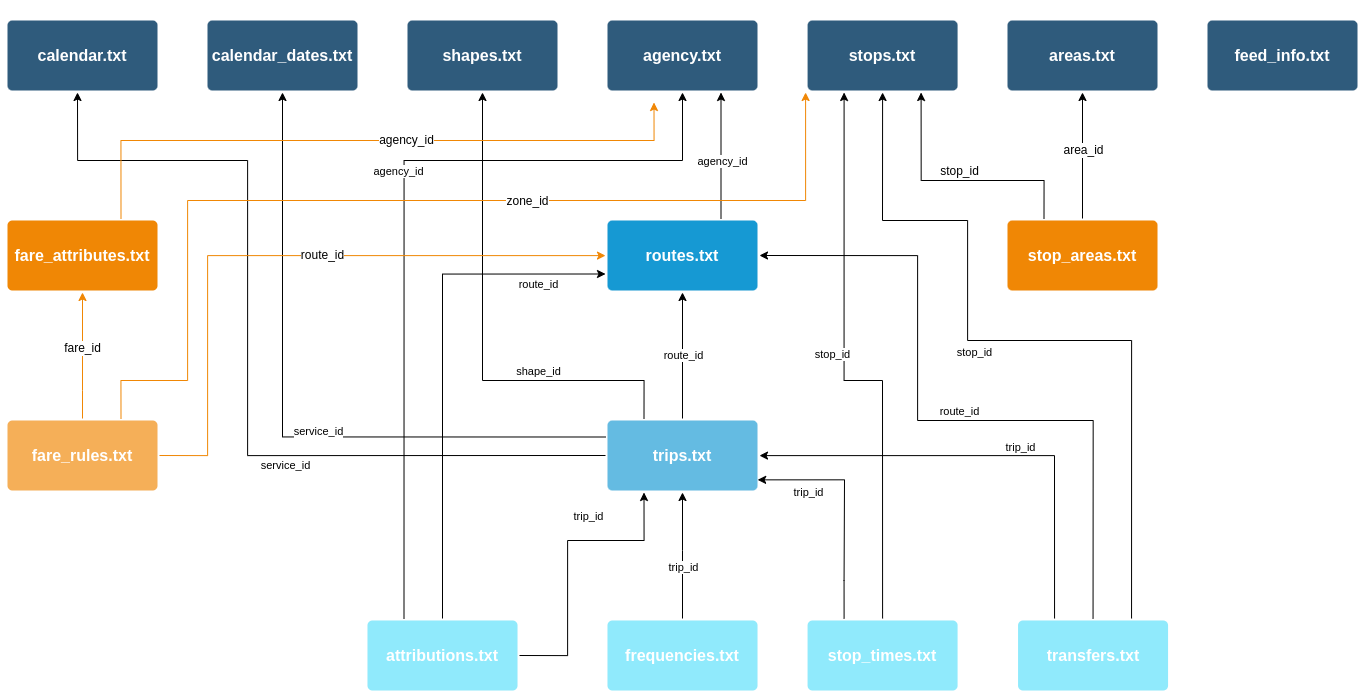
\includegraphics[width=1.0\textwidth]{images/GTFS_Diagram.png}
    \caption{GTFS Dependencies}
    \label{fig:figure1}
\end{figure}

\begin{justify}
The above figure highlight dependencies between GTFS feeds foreseen in the standard [1] and will be a helpful reference in this manual.
\end{justify}


\definecolor{gray}{rgb}{0.9,0.9,0.9}

\newpage
\subsection{GAIA Configuration}

\begin{justify}
There are two configuration files that are required by the application in order to work properly:
\begin{itemize}
\item \textbf{gaia.cfg}: with all global settings
\item \textbf{gtfs.cfg}: to be customised accordingly with data set and application needs.
\end{itemize}
\end{justify}

\subsubsection{Settings in \textbf{gaia.cfg}}

\begin{justify}
This configuration file contains all global settings such as directories to be used and settings for both logging and parser.
Let's see all of this sections in details starting from \textbf{\textit{global}}.
\end{justify}

\begin{small}
\begin{lstlisting}[backgroundcolor=\color{gray},frame=single]
global = {
  src_dir="gtfs_in/";
  dst_dir="gtfs_out/";
  feed_extension=".txt"
 
  logging = { ... };
  parser  = { ... };
}
\end{lstlisting}  
\end{small}

\begin{itemize}
\item \textbf{src\_dir}: specify \textit{source directory} where to find original \textbf{\textit{GTFS feeds}}.
\item \textbf{dst\_dir}: specify \textit{destination directory} used to write GTFS output feeds once all filters have been applied.
\item \textbf{feed\_extension}: file extension type for the \textbf{\textit{GTFS feeds}}.
\item \textbf{logging}: subsection containing general logging general settings.
\item \textbf{parser}: subsection containing general parser general settings.
\end{itemize}

\newpage
\subsubsection{global.logging}

In this subsection we can find all global settings for the logger.

\begin{small}
\begin{lstlisting}[backgroundcolor=\color{gray},frame=single]
  logging = {
    log_directory="log/";
    log_filename="_gaia.log";
    log_enable_console=true  
  };
\end{lstlisting} 
\end{small} 
\begin{itemize}
\item \textbf{log\_directory}: specify the directory where to write outputl logs. 
If specified directory does not exists it will be created.  
\item \textbf{log\_filename}: suffix appended to each log filename, more in general the\newline 
application will generate a new log file at each run and format used \newline
is \textbf{YYYYmmGGHHMMSS}, so final log filename will have the following\newline
form \textit{20221120104006\_gaia.log} where we have information about the\newline 
date \textbf{2022/11/20} and time \textbf{10:40:06} in which log have been generated.
\item \textbf{log\_enable\_console}: enable or disable log on standard output.
\end{itemize}

\newpage
\subsubsection{global.parser}

In this subsection are listed settings for the csv parser, such information will be used to initialize \href{https://github.com/fe-dagostino/libcsv}{\textit{\textbf{libcsv}}}.

\begin{small}
\begin{lstlisting}[backgroundcolor=\color{gray},frame=single]
  parser = {
    delimeter        = ",";
    quote            = "\"";
    eol              = "\n";
    comment          = "#";
    whitespaces      = "\a\b\t\v\f\r\n";
    skip_whitespaces = true;
    trim_all         = true;
    allow_comments   = false;
  };
\end{lstlisting}
\end{small}

\begin{itemize}
\item \textbf{delimeter}: characther used as \textit{field delimeter} when parsing \textit{csv} \textit{row}
\item \textbf{quote}: characther used as \textit{quote delimeter} when parsing the single \textit{field} in a \textit{row}
\item \textbf{eol}: End Of Line character used to identify when a \textit{row} has ended
\item \textbf{comment}: \textit{csv} standard do not make any mention for remarks inside the \textit{csv} itself, anyway the parser have this capability. 
\item \textbf{whitespaces}: define the list of whitespaces
\item \textbf{skip\_whitespaces} = \textit{enable}/\textit{disable} skip whitespaces. When true all whitespaces will be not anymore present in the \textit{output}.
\item \textbf{trim\_all}: \textit{enable}/\textit{disable} \textit{trim all}. When enabled all spaces at before and after a field will be removed unless the field is quoted.
\item \textbf{allow\_comments}: \textit{enable}/\textit{disable} comments inside the \textit{csv}.
\end{itemize}

\newpage
\subsubsection{Settings in \textbf{gtfs.cfg}}

\begin{justify}
While \textit{gaia.cfg} have a fixed number of subsections, this is not the case for \textit{gtfs.cfg} in which we can have a variable number of subsection describing feeds, dependencies and filters to be applied.
This file have been organized in two main parts:
\begin{itemize}
\item \textbf{feeds}: containing the exhaustive list of all \textit{csv} files that we want to process. Here we shall list both standard GTFS files as well as extra files not included in the standard that we want to process with GAIA, assuming that those files are also in \textit{csv} format.\newline
\textbf{Note}: that files not listed here will be not included in the output.
\item \textbf{feeds.name}: we should have as many as we have listed in \textbf{feeds}
\end{itemize}
Let's see an example in order to provide details for all parameters and to clarify usage.
\end{justify}

\begin{small}
\begin{lstlisting}[backgroundcolor=\color{gray},frame=single]
gtfs =
{
  feeds = ( 
            { 
              name          = "agency"
              filename      = "agency.txt";
              presence      = "required";
              dependencies  = [];
            },
            { 
              name          = "routes";
              filename      = "routes.txt";
              presence      = "required";
              dependencies  = ["agency"];
            },
            { 
              name          = "trips";
              filename      = "trips.txt";
              presence      = "required";
              dependencies  = ["calendar","calendar_dates"];
            },
..
...           
\end{lstlisting}
\end{small}

\begin{justify}
In the above example we have 3 feeds listed and for each one of them have been provided the following information:
\begin{itemize}
\item \textbf{name}: this is the name we will use to specify rules on this feed;
\item \textbf{filename}: used to specify filename for the feed;
\item \textbf{presence}: determine if such file must be present \textit{"required"}, is required under certain conditions \textit{"conditional"} or if not essential and then \textit{"optional"}. Such field have been set accordingly with the GTFS specification;
\item \textbf{dependencies}: the list of feeds to be processed before to start processing current feed. In the above, \textit{"agency"} do not have any dependency, \textit{"routes"} will be processed only after \textit{"agency"} and  \textit{"trips"} will be processed only after both \textit{"calendar"} and \textit{"calendar\_dates"}.
\end{itemize}
\textbf{Note}: feeds subsection have been already populated and comprises all files in \textit{Figure \ref{fig:figure1}} with related dependencies, so in general, starting from a default \textit{gtfs.cfg} users should remove all files not needed and eventually add extra files if any.
\end{justify}

\begin{justify}
Since we listed all \textit{feeds} required by the application, now let's check what we have to specify for each \textit{feed}. Again the best way to start is from default \textit{gtfs.cfg}, removing all unnecessary field and updating rules as for our needs.
\end{justify}

\begin{justify}
Moving forward with the example, just we just take agency.txt in order to explain how GAIA works.
\end{justify}

\begin{small}
\begin{lstlisting}[backgroundcolor=\color{gray},frame=single]
 // agency.txt
  agency = {
    // Mandatory fields required for the input feed
    mandatory-fields = ["agency_id","agency_name","agency_url",
                        "agency_timezone"];
    output-header    = ["agency_id","agency_name","agency_url",
                        "agency_timezone","agency_lang",
                        "agency_phone","agency_fare_url",
                        "agency_email"];
    filter-fields    = ["agency_id","agency_name","agency_url",
                        "agency_timezone"];
    //default-content  = ( [], [] );
    
    ...
    ....

  };
\end{lstlisting}
\end{small}

\newpage
\begin{justify}
As described before each subsection start with the name of the feed we listed in the first subsection "feeds", so here in our example we have "agency = \{..." and then all details:
\begin{itemize}
\item \textbf{mandatory-fields}: the list of all mandatory field that expected in the agency.txt provided as input.
\item \textbf{output-header}: the list of all fields for agency.txt once processed. Fields will be exported in the same order as listed in here, for many applications this is not important but for some use cases it is a constraint to have a specific order.
\item \textbf{filter-fields}: here the list of fields that GAIA should process. Listed order will match with processing order and this is something to keep in mind if we have filters that use other fields values to build the content. For each single field listed in this GAIA will expect to find the next level of details that correspond to which filters to apply and in which sequence.
\item \textbf{default-content}: if specified file (in the above example agency.txt) do not exist in the input set, then GAIA will create such file with a default content. Could be possible to specify more than one row.
\end{itemize}

It is foreseen one more optional section here that allow to enable specific functionalities most of the time related to dependencies between feeds. Agency do not have any dependecy, so in this specific case we don't have any function associated to this specific feed, but there are other feeds in which this section can be really important, files such as \textit{trips.txt} in which we have many dependencies from other files.

Here how the optional "\textit{processing}" looks like:

\begin{small}
\begin{lstlisting}[backgroundcolor=\color{gray},frame=single]
  processing = {
      enable = [ "find_orphan_routes", "find_orphan_services",
                 "find_orphan_shapes", "delete_unused_shapes", 
                 "optimize_shapes_usage" ];
    
      //  Raise a log message when for the specific trip is not 
      //  possible to retrieve route information, 
      //  since specified route_id do not exist in routes.
      find_orphan_routes = {
        level  = "error";
        params = [];
      };
      ..
      ...
  } 
\end{lstlisting}
\end{small}

The "\textit{processing}" section allow us to enable specific functionalities for the csv files we are currently processing.
It is important to know that each \textit{csv} files is subject to two different phases:
\begin{itemize}
\item \textbf{parsing}: operations performed during parsing. More in details as soon as a new \textit{row} have been parsed, GAIA check for filters chains and apply all of them to such row.
\item \textbf{post-parsing}: starting from the assumption that rows in a \textit{csv} files can be disordered, then we have some operations that can be performed only once we have \textit{csv} file and its dependencies fully parsed. 
\end{itemize}

All functionalities available in post-parsing will be detailed forward in the this document.

Coming back to "agency.txt" example, let's complete to describe how it works describing \textit{filter\_chains} and \textit{filters}.

\begin{small}
\begin{lstlisting}[backgroundcolor=\color{gray},frame=single]
 // agency.txt
  agency = {
    ..
    ...
    filter-fields    = ["agency_id","agency_name","agency_url",
                        "agency_timezone"];    
    
    agency_id = {
      filters_chain= ("empty","length","unique");
      empty = {
        level  = "error";
        stop   = true;       // do not process next filter
        params = ["false"];
      };
      length = {
        level  = "error";
        stop   = false;
        params = ["-1","30"];
      };
      unique = {
        level  = "error";
        stop   = false;
        params = [];
      };
    };

    agency_name = {
      filters_chain= ("empty","length");
      empty = {
        level  = "error";
        stop   = true;      // do not process next filter
        params = ["false"];
      };
      length = {
        level  = "error";
        stop   = false;
        params = ["1","50"];
      };    
    };

    agency_url = {
      filters_chain= ("empty","length");
      empty = {
        level  = "error";
        stop   = true;      // do not process next filter
        params = ["false"];
      };
      length = {
        level  = "error";
        stop   = false;
        params = ["7","1000"];
      };    
    };

    // Valid Time Zones are listed at the following url.
    // https://en.wikipedia.org/wiki
    // /List_of_tz_database_time_zones
    agency_timezone = {
      filters_chain= ("empty");
      empty = {
        level  = "error";
        stop   = true;      // do not process next filter
        params = ["false"];
      };
    };

  };
\end{lstlisting}
\end{small}

\newpage
Accordingly with \textit{filter-fields} GAIA is expecting to find out details for all four field listed here and more in details are required:
- a subsection with the name of the field
- the list of filters to be applied to such field
- filters' parameters
So, let's take an example providing details on each part and then we will have all the basis to customise our \textit{gtfs.cfg}.\newline

From the about let's take the first field "agency\_id":

\begin{small}
\begin{lstlisting}[backgroundcolor=\color{gray},frame=single]
 // agency.txt
  agency = {
    ..
    ...
    filter-fields    = ["agency_id","agency_name","agency_url",
                        "agency_timezone"];    
    
    agency_id = {
      filters_chain= ("empty","length","unique");
      empty = {
        level  = "error";
        stop   = true;       // do not process next filter
        params = ["false"];
      };
      length = {
        level  = "error";
        stop   = false;
        params = ["-1","30"];
      };
      unique = {
        level  = "error";
        stop   = false;
        params = [];
      };
    };
\end{lstlisting}
\end{small}

The subsection in \textit{agency} start with the the name of the field \textit{agency\_id} and contains the following elements:
\begin{itemize}
\item \textbf{filters\_chain}: the list of \textit{filters} to be applied to each value under \textit{agency\_id} in \textit{agency.txt}. \textbf{Note}: that filters will be applied from left to right, so in this example "\textit{empty}" will be the first filter, "\textit{length}" the second and "\textit{unique}" the third. Moreover, the same filter can be repeated and this can be useful in case we make some composition.
\item \textbf{\textit{filter}}: for each \textit{filter} listed in \textit{filters\_chain} we will have one more subsection with its configuration:
\begin{itemize}
\item \textbf{level}: can be one of the following values "\textit{debug}", "\textit{info}", "\textit{warning}", "\textit{error}", "\textit{raw}". Values do not affect the behaviours, but it is useful in the final report or for automatic system. This is completely in charge to the user to classify the severity level for the specific check. In this case since "\textit{agency\_id}" is a \textit{key} element for \textit{agency.txt} it have been classified as \textit{error}. If there is an automatic system reading the results, then can stop the process in presence of errors and send email or notifications in order to fix it.
\item \textbf{stop}: can be \textit{true} that means to do not proceed with other filters since no make sense to check other rules on a field that already have such error; \textit{false}, it means continue anyway even in cases of failure continue with next filter. Just note that each failure will generate log information and in some cases can be convenient to keep logs with necessary information. In the above example, we are telling to GAIA to stop executing next filter in case the field is \textit{empty} since no make sense to check length on an empty field or to check if such field is unique.
\item \textbf{params}: here will be possible to provide a parameters list for the filter. Each filter has its own parameters or no parameters at all.
\end{itemize}
\end{itemize}
\end{justify}

\newpage
\section{Filters}

Filters are organized by version in order to know since which version a specific filter is available.

\subsection{Version 0.2.0}

\subsubsection{empty}
\begin{justify}
Check emptiness for the specified field.
\end{justify}

\begin{itemize}
\item \textbf{level}: ["\textit{debug}" $|$ "\textit{info}" $|$ "\textit{warning}" $|$ "\textit{error}" $|$ "\textit{raw}"]
\item \textbf{stop}: [ \textit{true} $|$ \textit{"false"} ]
\item \textbf{params}: 
  \begin{itemize}
  \item expected 1 (one) parameter 
  \item 1° parameter: [ \textit{"true"} $|$ \textit{"false"} ]
    \begin{itemize}
    \item \textbf{true}: expected that such field will be empty, then if populated with any information filter will fail
    \item \textbf{false}: expected that such field will be not empty, then if no data will be found filter will fail
    \end{itemize}
  \end{itemize}
\end{itemize}


\subsubsection{length}
\begin{justify}
Check if specified field length is in the specified range of (min,max).
\end{justify}

\begin{itemize}
\item \textbf{level}: ["\textit{debug}" $|$ "\textit{info}" $|$ "\textit{warning}" $|$ "\textit{error}" $|$ "\textit{raw}"]
\item \textbf{stop}: [ \textit{true} $|$ \textit{"false"} ]
\item \textbf{params}: 
  \begin{itemize}
  \item expected 2 (two) parameters respectively "\textit{min}" and "\textit{max}"
  \item 1° parameter: [ "-1" $|$ "\textit{min value}" ]
    \begin{itemize}
    \item \textbf{"-1"}: min value will be ignore
    \item \textbf{\textit{value}}: expected minimum number of characters for this field
    \end{itemize}
  \item 2° parameter: [ "-1" $|$ "\textit{max value}" ]
    \begin{itemize}
    \item \textbf{"-1"}: max value will be ignore
    \item \textbf{\textit{value}}: expected maxmum number of characters for this field
    \end{itemize}
  \end{itemize}
\end{itemize}


\subsubsection{swap}
\begin{justify}
Swap two items, supposing A and B the two values, all occurrence of 'A' will be replaced with 'B' and all occurrence of 'B' with replaced with 'A'. 
\end{justify}

\begin{itemize}
\item \textbf{level}: ["\textit{debug}" $|$ "\textit{info}" $|$ "\textit{warning}" $|$ "\textit{error}" $|$ "\textit{raw}"]
\item \textbf{stop}: [ \textit{true} $|$ \textit{"false"} ]
\item \textbf{params}: 
  \begin{itemize}
  \item expected 2 (two) parameters respectively "\textit{value A}" and "\textit{value B}"
  \item 1° parameter: "\textit{A}"
  \item 2° parameter: "\textit{B}"
  \end{itemize}
\end{itemize}


\subsubsection{replace}
\begin{justify}
An extension to \textit{swap function} for multiple replacements.
Specify a list of replacements for specific field 'A' will be replaced with 'B', 'C' will be replaced with 'D' and so on ...
Moreover is also possible to specify a default value will be addressed with '*' that, if present, will replace all other occurrence with a default value.
\end{justify}

\begin{itemize}
\item \textbf{level}: ["\textit{debug}" $|$ "\textit{info}" $|$ "\textit{warning}" $|$ "\textit{error}" $|$ "\textit{raw}"]
\item \textbf{stop}: [ \textit{true} $|$ \textit{"false"} ]
\item \textbf{params}: 
  \begin{itemize}
  \item expected N parameters
  \item 1° parameter: [ "A$|$B" ]
  \item 2° parameter: [ "C$|$D" ]
  \item N° parameter: [ "*$|$E" ]
  \end{itemize}
\end{itemize}


\newpage
\subsubsection{substring}
\begin{justify}
Specify a list of replacement for specific field. In a field containing '\textbf{a}', this last value will be replaced with '\textbf{b}'.\newline
Eg. For \textit{block\_id} we can specify the following two paramenters "/$|$.", "\textbackslash$|$\_\_", then supposing to have a \textit{block\_id} defined as "T100\textbf{/}T200" then it will be modified in "T100\textbf{.}T200", also if \textit{block\_id} contains "T100\textbf{\textbackslash}T200" it will be modified in "T100\textbf{\_\_}T200".
\end{justify}

\begin{itemize}
\item \textbf{level}: ["\textit{debug}" $|$ "\textit{info}" $|$ "\textit{warning}" $|$ "\textit{error}" $|$ "\textit{raw}"]
\item \textbf{stop}: [ \textit{true} $|$ \textit{"false"} ]
\item \textbf{params}: 
  \begin{itemize}
  \item expected N parameters
  \item 1° parameter: [ "A$|$B" ]
  \item 2° parameter: [ "C$|$D" ]
  \item N° parameter: [ "*$|$E" ]
  \end{itemize}
\end{itemize}


\subsubsection{unique}
\begin{justify}
Specify that such field is a key value and must be unique in the file.
\end{justify}

\begin{itemize}
\item \textbf{level}: ["\textit{debug}" $|$ "\textit{info}" $|$ "\textit{warning}" $|$ "\textit{error}" $|$ "\textit{raw}"]
\item \textbf{stop}: [ \textit{true} $|$ \textit{"false"} ]
\item \textbf{params}: \textit{no parameters}
\end{itemize}


\subsubsection{concat}
\begin{justify}
Concatenate fields and string in order to obtain a new string that will replace field value. The following example for \textbf{trip\_headsign} params = ["route\_id"," - ","trip\_headsign"] will replace the content of \textbf{trip\_headsign} field with a concatenation of \textit{route\_id} plus the fixed string "\textit{ - }" plus \textit{trip\_headsign} value.
\end{justify}

\begin{itemize}
\item \textbf{level}: ["\textit{debug}" $|$ "\textit{info}" $|$ "\textit{warning}" $|$ "\textit{error}" $|$ "\textit{raw}"]
\item \textbf{stop}: [ \textit{true} $|$ \textit{"false"} ]
\item \textbf{params}: 
  \begin{itemize}
  \item expected N parameters
  \item 1° parameter: [ "\textit{field name}" $|$" \textit{string}" ]
  \item 2° parameter: [ "\textit{field name}" $|$" \textit{string}" ]
  \item N° parameter: [ "\textit{field name}" $|$" \textit{string}" ]
  \end{itemize}
\end{itemize}


\subsubsection{fix\_real}
\begin{justify}
Fix floating values to specified form in terms of decimal digits. So if a value appears with 20 decimal digits but decimal part is specified as 8 digits then such value will be truncated to 8 decimal digits.
\end{justify}

\begin{itemize}
\item \textbf{level}: ["\textit{debug}" $|$ "\textit{info}" $|$ "\textit{warning}" $|$ "\textit{error}" $|$ "\textit{raw}"]
\item \textbf{stop}: [ \textit{true} $|$ \textit{"false"} ]
\item \textbf{params}: 
  \begin{itemize}
  \item expected 1 (one) parameter
  \item 1° parameter: [ "decimal digits" ]
  \end{itemize}
\end{itemize}


\subsubsection{format}
\begin{justify}
Allow use of a regular expression in order to validate field value.
\end{justify}

\begin{itemize}
\item \textbf{level}: ["\textit{debug}" $|$ "\textit{info}" $|$ "\textit{warning}" $|$ "\textit{error}" $|$ "\textit{raw}"]
\item \textbf{stop}: [ \textit{true} $|$ \textit{"false"} ]
\item \textbf{params}: 
  \begin{itemize}
  \item expected 1 (one) parameter
  \item 1° parameter: [ "rexgex" ]
  \end{itemize}
\end{itemize}

\newpage
\subsubsection{expired}
\begin{justify}
Determine if date field compared with current date is already expired.
Due to usage of local time a valid Time Zone shall be provided.
A full list can be retrieved at the following URL: \href{https://en.wikipedia.org/wiki/List_of_tz_database_time_zones}{\textit{https://en.wikipedia.org/wiki/List\_of\_tz\_database\_time\_zones}}.
\end{justify}

\begin{itemize}
\item \textbf{level}: ["\textit{debug}" $|$ "\textit{info}" $|$ "\textit{warning}" $|$ "\textit{error}" $|$ "\textit{raw}"]
\item \textbf{stop}: [ \textit{true} $|$ \textit{"false"} ]
\item \textbf{params}: 
  \begin{itemize}
  \item expected 1 (one) parameter
  \item 1° parameter: [ "time zone" ]
  \end{itemize}
\end{itemize}


\subsubsection{ne}
\begin{justify}
The function check if current field is NE (not equal) to a specified field on the same row.
\end{justify}

\begin{itemize}
\item \textbf{level}: ["\textit{debug}" $|$ "\textit{info}" $|$ "\textit{warning}" $|$ "\textit{error}" $|$ "\textit{raw}"]
\item \textbf{stop}: [ \textit{true} $|$ \textit{"false"} ]
\item \textbf{params}: 
  \begin{itemize}
  \item expected 1 (one) parameter
  \item 1° parameter: [ "field name" ]
  \end{itemize}
\end{itemize}


\subsubsection{le}
\begin{justify}
The function check if current field is LE (\textbf{L}ess than or \textbf{E}qual) to a specified field on the same row.
\textbf{Note}: comparison is between strings, so even numeric values will be treated as string.
\end{justify}

\begin{itemize}
\item \textbf{level}: ["\textit{debug}" $|$ "\textit{info}" $|$ "\textit{warning}" $|$ "\textit{error}" $|$ "\textit{raw}"]
\item \textbf{stop}: [ \textit{true} $|$ \textit{"false"} ]
\item \textbf{params}: 
  \begin{itemize}
  \item expected 1 (one) parameter
  \item 1° parameter: [ "field name" ]
  \end{itemize}
\end{itemize}


\subsubsection{ge}
\begin{justify}
The function check if current field is GE (\textbf{G}reater than or \textbf{E}qual) to a specified field on the same row.
\textbf{Note}: comparison is between strings, so even numeric values will be treated as string.
\end{justify}

\begin{itemize}
\item \textbf{level}: ["\textit{debug}" $|$ "\textit{info}" $|$ "\textit{warning}" $|$ "\textit{error}" $|$ "\textit{raw}"]
\item \textbf{stop}: [ \textit{true} $|$ \textit{"false"} ]
\item \textbf{params}: 
  \begin{itemize}
  \item expected 1 (one) parameter
  \item 1° parameter: [ "field name" ]
  \end{itemize}
\end{itemize}


\newpage
\section{Functions}

Functions are defined and optimized at feeds level, so a function that is available for a specific file, not necessarily is available also for other files.

\subsection{Version 0.2.0 - trips.txt}


\subsubsection{"find\_orphan\_routes"}
\begin{justify}
Raise a log message when for a specific \textit{trip} is not possible to retrieve \textit{route} information, since specified \textit{route\_id} does not exist in \textit{routes.txt}.
\newline
\end{justify}


\subsubsection{"find\_orphan\_services"}
\begin{justify}
Raise a log message when for a specific \textit{trip} is not possible to retrieve \textit{service} information, since specified \textit{service\_id} does not exist in both \textit{calendar.txt} and \textit{calendar\_dates.txt}.
\end{justify}


\subsubsection{"find\_orphan\_shapes"}
\begin{justify}
Raise a log message when for a specific \textit{trip} is not possible to retrieve \textit{shape} information, since specified \textit{shape\_id} does not exist in \textit{shapes.txt}.
\end{justify}


\subsubsection{"delete\_unused\_shapes"}
\begin{justify}
Mark as \textit{deleted} all \textit{shape\_id} that are not linked with a \textit{trip\_id}. All of such \textit{shapes} will be excluded from output.
\end{justify}


\subsubsection{"optimize\_shapes\_usage"}
\begin{justify}
Merge all \textit{shapes} that are duplicated in \textit{shapes.txt} and replace the link in \textit{trips.txt}. This optimization, in some cases, can drastically reduce the size for \textit{shapes.txt}.
\end{justify}


\subsection{Version 0.2.0 - stop\_times.txt}

\subsubsection{"find\_orphan\_links"}
\begin{justify}
Raise a log message when for a specific \textit{trip} is not possible to retrieve \textit{stop} or \textit{trip} information, since specified \textit{stop\_id} or \textit{trip\_id} does not exist respectively in \textit{stops.txt} or \textit{trips.txt}.
\end{justify}


\subsection{Version 0.2.0 - shapes.txt}

\subsubsection{"check\_distance"}
\begin{justify}
Compute the distance for all the shapes replacing current values.\newline\newline
\textbf{Note}: be sure to enable this function only if you want to replace current values.
Take care that computed distance should be consistent also with \textit{stop\_times.txt}, so an error in \textit{shapes.txt} most likely means that such error is also present in \textit{stop\_times.txt}.\newline\newline
\textbf{Parameters}: only take one parameter in order to specify the number of decimal digits for the precision (\textit{default is 10 digits}).

\end{justify}

\end{document}

